\chapter{Project Structure}
\label{cha:project_structure}
This chapter aims to show the concrete structure and communication of a project, which implements the previously discussed authentication mechanisms.
The focus of this chapter is showing the effects of the different authentication mechanisms on the project itself.
For simplicity, this chapter does not handle topics like authorization, key management and user context sharing.
The visualizations are based on the backend of a flea market app.

\section{Flea Market App}
The flea market app is an Android App written in the programming language Kotlin.
The main features are buying, renting, and swapping items.
The user is authenticated using firebase authentication.
Therefore, he must present his access token to the Microsoft API Gateway with each request.
The backend of the app is based on the microservice architecture.
The microservices are mainly implemented in C\# using the ASP.Net Core framework.
Actually the backend contains the following services:
\begin{itemize}
	\item AdService
	\item UserService
	\item ChatService
	\item MediaService
	\item SubscriptionService
	\item ReportService
\end{itemize}
Each service has its own PostgreSQL database.
The services are hosted on Microsoft Azure using docker containers.
The AdService and the UserService will be used to show the communication within the deployment of the project using the discussed authentication mechanisms.

\section{Communication among the Components}
Figure~\ref{fig:deployment_communication} visualizes the communication among the components for an example use case.
In this example, the user fetches all ads in his surroundings.
%Possibly wordy sentence
Therefore the AdService is used to retrieve the ads from the database, and the UserService is needed to preview information about the seller.
The following components are necessary for the declared use case:
\begin{description}
	\item[Android App:] The Android App is the User Interface for the client, that allows the users to access the functionalities of the services.
		The requests sent by the Android App are sent in beyond of the user.
	\item[Firebase:] The Firebase service is responsible for validating the access tokens transferred by the users.
		The app also communicates with the Firebase service to get an access token, but this is done earlier.
	\item[API Gateway:] The API Gateway is the only entry point into the deployment.
		Therefore the API Gateway is the only component directly communicating to the Android App.
	\item[AdService:] The AdService is responsible for managing the users' ads.
	\item[UserService:] The AdService is responsible for all management tasks regarding the users' data.
\end{description}

\begin{figure}
	\centering
	\tikzset{
		every picture/.append style={
			transform shape,
			scale=0.85
		}
	}
	\begin{sequencediagram}
		\newthread{app}{:Android App}{}
		\newinst[1]{gateway}{:API Gateway}{}
		\newinst[1]{fa}{:Firebase}{}
		\newinst[1]{as}{:AdService}{}
		\newinst[1]{us}{:UserService}{}

		\begin{call}{app}{\shortstack{request$_{1}$}}{gateway}{response$_1$}
			\begin{call}{gateway}{access token}{fa}{validity}
			\end{call}
			\begin{sdblock}{if}{validity == true}
				\begin{call}{gateway}{request$_1$}{as}{response$_1$}
					\begin{call}{as}{request$_2$}{us}{reponse$_2$}
					\end{call}
				\end{call}
			\end{sdblock}
		\end{call}
	\end{sequencediagram}
	%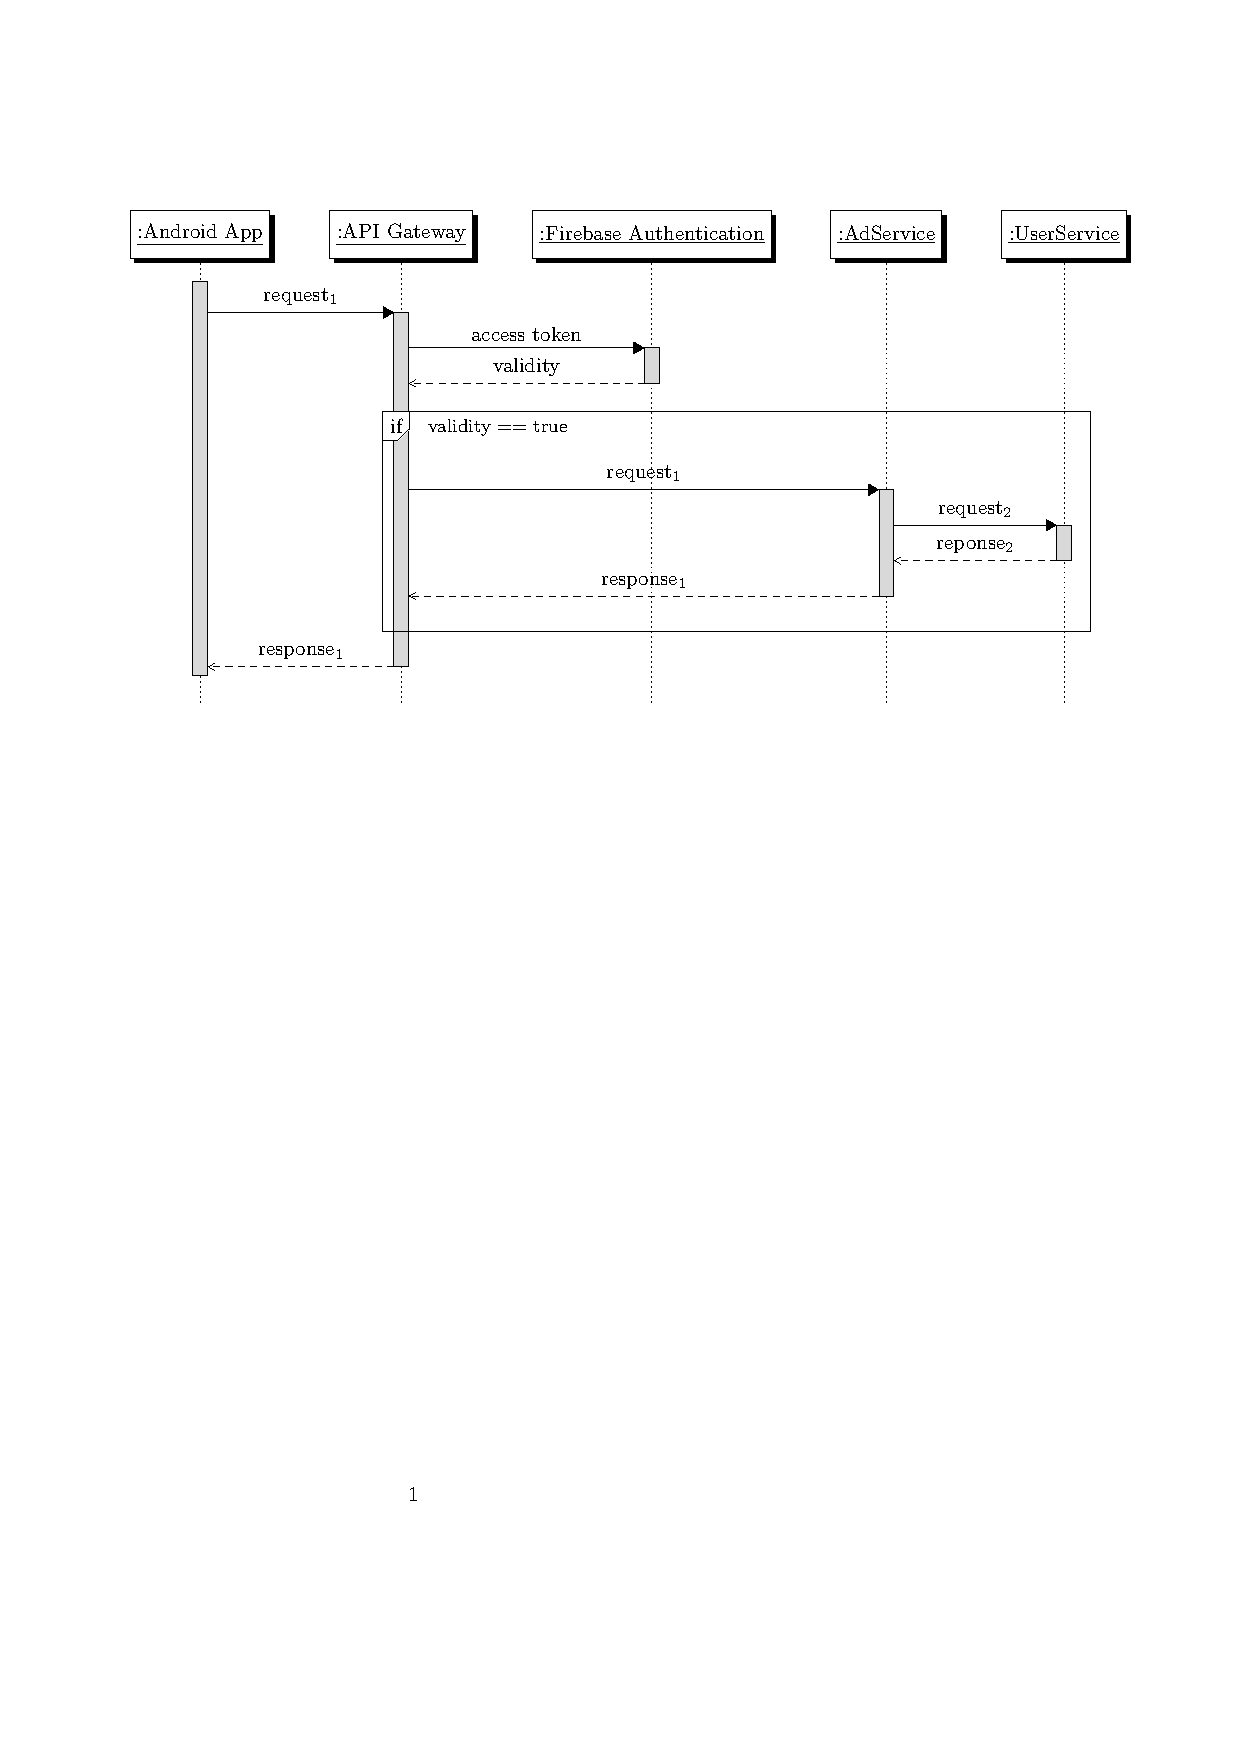
\includegraphics[width=0.7\textwidth]{images/project-structure/sequence-structure.pdf}
	\caption{Communication among the components of the flea market app}
	\label{fig:deployment_communication}
\end{figure}

\subsection{Workflow using mTLS}
\begin{enumerate}
	\item[1.] The client sends an API request to the Microsoft API Gateway using the Android App.
		The communication between the API Gateway and the app is secured using HTTPS.
		Therefore the server is authenticated to the client using TLS.
		The client is authenticated to the server by embedding a firebase access token within the Authorization header.
	\item[2.] The API Gateway sends the received token to the Firebase service for the validation.
		This procedure is defined as a policy within the policy file of the API Gateway.
		\newpage
	\item[3.] The Firebase service returns the information whether the presented token is valid or not.
	\item[4.] When the client provides a valid access token, the request of the client is forwarded to the \textbf{AdService}.
		The communication between the API Gateway and the \textbf{AdService} is secured using mTLS.
%Unclear antecedent
		This means both parties have to present a certificate signed by a trusted CA.
		Therefore the webserver of the \textbf{AdService} has to be configured to allow or even require Client Certificates.
	\item[5.] After processing the request from the API Gateway, the \textbf{AdService} sends a request to the \textbf{UserService} to retrieve additional information about the owner of the ad.
		The communication between the \textbf{UserService} and the \textbf{AdService} is also protected using mTLS.
		Therefore the \textbf{AdService} implements the same authentication mechanism as the \textbf{UserService}.
		The certificate is appended to the request using an HTTPClient, which is injected to the Controller of the WebService using Dependency Injection.
	\item[6.] When the \textbf{UserService} processed the request, it responds to the request.
		The response does not require performing the authentication again since the TCP connection between the \textbf{AdService} and the \textbf{UserService} is still opened.
	\item[7.] After the \textbf{AdService} processed the response from the \textbf{UserService}, it uses the opened connection with the API Gateway and transfers its response.
	\item[8.] The API Gateway forwards the response from the \textbf{AdService} to the Android App.
		This connection is still secured using TLS. 
		The app can now process the response and present the requested information to the user.
\end{enumerate}

\subsection{Workflow using JWT}
The workflow using JWT and the workflow using mTLS are pretty similar.
Therefore, only the steps which differ between the mechanisms are described again.
\begin{enumerate}
	\item[4.] The request from the client is forwarded to the \textbf{UserService}. 
		Therefore the API Gateway has to create a valid JWT to communicate with the \textbf{UserService}.
		The JWT, which is signed using the private key of the API Gateway, is transferred within the Authorization header.
	\item[5.] The \textbf{AdService} has to retrieve additional information from the \textbf{UserService}.
		Now the \textbf{AdService} has to present his JWT to the \textbf{UserService}.
% Unclear antecedent
		This is done by embedding the JWT within the request's Authorization header.
		If the \textbf{AdService} does not know the certificate of the \textbf{UserService}, it will deny the request and ask the \textbf{AdService} to present its certificate.
%Possibly wordy sentence
		In this case, the request is repeated, and the certificate of the \textbf{AdService} is transferred by appending the certificate as client certificate to the request.
\end{enumerate}

\section{Implementation Details}

\subsection{mTLS} \label{sec:impl_details_mtls}
As already discussed in chapter~\ref{cha:authentication_mechanisms}, the implementation of mutual TLS does not require much logic on the service side.
The best way to implement mTLS in an ASP.Net Core API is using the \textbf{Microsoft.AspNetCore.Authentication.Certificate} library.
It provides the mechanism to add certificate authentication as \textbf{AuthenticationScheme} and implement custom \textbf{CertificateAuthenticationEvents}.
The \textbf{CertificateAuthorityService}, implements the interface \textbf{ICertificateAuthorityService} which is shown in listing~\ref{lst:ICertificateAuthorityService}.
It provides features to manage a custom certificate truststore and validate certificates using this truststore.
An instance of the \textbf{CertificateAuthorityService} is injected to the \textbf{CertificateAuthenticationEvents}.
The dependency injection is managed by the \textbf{Microsoft.Extensions.DependencyInjection} library.
The \textbf{UseAuthentication} and \textbf{UseAuthorization} functions of the \textbf{ApplicationBuilder} have to be called to use the created \textbf{AuthenticationScheme}.
The functions of the API Controllers have to be marked with the \textbf{[Authorize]} annotation to perform the declared authentication mechanism.

The client has to attach his certificate to the request.
In ASP.Net this is done, by creating a custom \textbf{HTTPHandler}, and setting the \textbf{ClientCertificate} property.
The \textbf{HTTPHandler} is then used to create a \textbf{HTTPClient}, which is used to perform the requests.
It is good-practice to create the \textbf{HTTPClient} once and then inject it into the Controllers using dependency injection.
% Unclear antecedent
This helps improve the performance and especially prevents the service certificate from being parsed multiple times.

\noindent \begin{minipage}{\linewidth}
	\begin{CsCode}[label={lst:ICertificateAuthorityService}, caption={ICertificateAuthorityService interface, which is implemented by the injected CertificateAuthorityService},captionpos=b]
		public interface ICertificateAuthorityService {
			public void AppendCertificate(X509Certificate2 certificate);
			public bool ValidateCertificate(X509Certificate2 certificate);
		}
	\end{CsCode}
\end{minipage}

\subsection{JWT}
The best way to implement mutual authentication using self-signed JWTs in ASP.Net Core is a custom middleware.
A custom middleware provides the possibility to perform actions on the receiving request before the API Controllers handle them.
The \textbf{JWTAuthenticationMiddleware} validates the JWTs and certificates of all received requests.
The validation is performed like it is shown in algorithm~\ref{alg:jwt}.
When a client certificate is transferred within the TLS handshake, it is checked using a service that implements the \textbf{ICertificateAuthorityService}, which was shown in listing~\ref{lst:ICertificateAuthorityService}.
If the certificate is valid, it is mapped to the issuer of the certificate within a custom truststore of the \textbf{JWTValidationService}.
The \textbf{JWTValidationService} implements the \textbf{ITokenValidationService} interface which is shown in listing~\ref{lst:ITokenValidationService}.
Both the \textbf{CertificateAuthorityService} and the \textbf{JWTValidationService} are injected into the \textbf{Invoke} function of the \textbf{JWTAuthenticationMiddleware} using dependecy injection.

\noindent \begin{minipage}{\linewidth}
	\begin{CsCode}[label={lst:ITokenValidationService}, caption={ITokenValidationService interface, which is implemented by the injected JWTValidationService},captionpos=b]
		public interface ITokenValidationService {
			public void PutIntoTruststore(X509Certificate2 certificate);
			public bool ContainsIssuerInTruststore(String issuer);
			public bool ValidateTokenWithTruststore(String token, string issuer);
		}
	\end{CsCode}
\end{minipage}

The client has to implement the logic for creating JWTs and attaching them to the requests within the Authorization header.
The JWTs are created, using the \textbf{JWTCreatorService} that implements the \textbf{ITokenCreatorService} which is shown in~\ref{lst:ITokenCreatorService}.
The \textbf{JWTCreatorService} and a \textbf{HTTPClient} are injected to the API Controllers using dependency injection.
The Controllers can choose between two clients, one containing the service certificate and one that does not contain a certificate.
In both cases, the Controller has to use the \textbf{JWTCreatorService} to create a JWT and append it to the Authorization header of each request.
The header and the body of an authentication JWT, created by the \textbf{JWTCreatorService} is shown in figure~\ref{fig:jwt_en_decoded}.

\noindent \begin{minipage}{\linewidth}
	\begin{CsCode}[label={lst:ITokenCreatorService}, caption={ITokenCreatorService interface, which is injected to the API Controllers},captionpos=b]
		public interface ITokenCreatorService {
			public string CreateToken(string audience);
			public string CreateToken(string audience, TimeSpan validityPeriod);
		}
	\end{CsCode}
\end{minipage}

\begin{figure}
	\begin{centering}
	\end{centering}
	\textcolor{red}{eyJhbGciOiJSUzI1NiIsImtpZCI6IkYwMURFNTBCNTU5MzVBQ0VEOUNDNzdCRjR\\FMjY5NkVDOTE4MUI5NjkiLCJ0eXAiOiJKV1QifQ}.
	\textcolor{blue}{eyJuYmYiOjE2NDU1MjU5MjM\\sImV4cCI6MTY0NTUyNjIyMywiaXNzIjoic2VydmljZTEuc3dhcGluZG8uY29tIiwiYXV\\kIjoic2VydmljZTIuc3dhcGluZG8uY29tIn0}.
	\\ 
	\begin{Verbatim}[commandchars=\\\{\}]
\textcolor{red}{\{} 
	\textcolor{red}{"alg": "RS256",}
	\textcolor{red}{"kid": "F01DE50B55935ACED9CC77BF4E2696EC9181B969",}
	\textcolor{red}{"typ": "JWT"} 
\textcolor{red}{\}}
\textcolor{blue}{\{} 
	\textcolor{blue}{"nbf": 1645525923,}
	\textcolor{blue}{"exp": 1645526223,}
	\textcolor{blue}{"iss": "service1.swapindo.com",}
	\textcolor{blue}{"aud": "service2.swapindo.com"} 
\textcolor{blue}{\}}
	\end{Verbatim}
	\caption{Header and Payload of a JWT, created by the JWTCreatorService}
	\label{fig:jwt_en_decoded}
\end{figure}

\begin{algorithm}[H]
	\caption{Pseudocode of the request validation using self-signed JWTs}\label{alg:jwt}
	\begin{algorithmic}
		\State $certificate \gets request.Connection.ClientCertificate$
		\State $token \gets request.Headers[Authorization]$
		\State $missingCertificate \gets false$

		\If{$token$ is $null$}
		\State $response.StatusCode \gets 403Forbidden$
		\State $authenticated \gets false$
		\Else
		\State $issuer \gets null$
		\If{$certificate$ is not $null$ \&\& $certificate$ is $trusted$} 
		\State $putCertificateIntoTruststore$($x$)
		\State $issuer \gets certificate.subject$
		\Else
		\If{$containsIssuerInTruststore(token.issuer)$}
		\State $issuer \gets token.issuer$
		\Else
		\State $missingCertificate \gets true$
		\EndIf
		\EndIf

		\If{$issuer$ is not $null$ \&\& $validateJWT(token)$ is $valid$}
		\State $authenticated \gets true$
		\Else
		\If{$missingCertificate$ is $true$}
		\State $response.StatusCode \gets 401Unauthorized$
		\Else
		\State $response.StatusCode \gets 403Forbidden$
		\EndIf
		\State $authenticated \gets false$
		\EndIf
		\EndIf
	\end{algorithmic}
\end{algorithm}

\section{Conclusion}
This chapter showed a concrete project which implements the previously discussed authentication concepts.
Furthermore, some implementation details were shown to give an idea of how the concepts can be implemented.
The implementation also proved that the authentication mechanism using self-signed JWTs requires more code than the implementation of mTLS.

The concrete implementation of the discussed authentication mechanisms differs depending on the programming language and the used technologies.
The main target was clarifying which tasks have to be performed by the services when the compared authentication mechanisms are implemented.
